\pdfminorversion=4
\documentclass[aspectratio=169]{beamer}

\mode<presentation>
{
  \usetheme{default}
  \usecolortheme{default}
  \usefonttheme{default}
  \setbeamertemplate{navigation symbols}{}
  \setbeamertemplate{caption}[numbered]
  \setbeamertemplate{footline}[frame number]  % or "page number"
  \setbeamercolor{frametitle}{fg=white}
  \setbeamercolor{footline}{fg=black}
} 

\usepackage[english]{babel}
\usepackage[utf8x]{inputenc}
\usepackage{tikz}
\usepackage{courier}
\usepackage{array}
\usepackage{bold-extra}
\usepackage{minted}
\usepackage[thicklines]{cancel}
\usepackage{fancyvrb}

\xdefinecolor{dianablue}{rgb}{0.18,0.24,0.31}
\xdefinecolor{darkblue}{rgb}{0.1,0.1,0.7}
\xdefinecolor{darkgreen}{rgb}{0,0.5,0}
\xdefinecolor{darkgrey}{rgb}{0.35,0.35,0.35}
\xdefinecolor{darkorange}{rgb}{0.8,0.5,0}
\xdefinecolor{darkred}{rgb}{0.7,0,0}
\definecolor{darkgreen}{rgb}{0,0.6,0}
\definecolor{mauve}{rgb}{0.58,0,0.82}

\title[2021-09-27-julia-workshop-awkward]{How an Awkward Array/Julia bridge can introduce HEP to Julia}
\author{Jim Pivarski}
\institute{Princeton University -- IRIS-HEP}
\date{September 27, 2021}

\usetikzlibrary{shapes.callouts}

\begin{document}

\logo{\pgfputat{\pgfxy(0.11, 7.4)}{\pgfbox[right,base]{\tikz{\filldraw[fill=dianablue, draw=none] (0 cm, 0 cm) rectangle (50 cm, 1 cm);}\mbox{\hspace{-8 cm}\includegraphics[height=1 cm]{princeton-logo-long.png}\hspace{0.1 cm}\raisebox{0.1 cm}{\includegraphics[height=0.8 cm]{iris-hep-logo-long.png}}\hspace{0.1 cm}}}}}

\begin{frame}
  \titlepage
\end{frame}

\logo{\pgfputat{\pgfxy(0.11, 7.4)}{\pgfbox[right,base]{\tikz{\filldraw[fill=dianablue, draw=none] (0 cm, 0 cm) rectangle (50 cm, 1 cm);}\mbox{\hspace{-8 cm}\includegraphics[height=1 cm]{princeton-logo.png}\hspace{0.1 cm}\raisebox{0.1 cm}{\includegraphics[height=0.8 cm]{iris-hep-logo.png}}\hspace{0.1 cm}}}}}

% Uncomment these lines for an automatically generated outline.
%\begin{frame}{Outline}
%  \tableofcontents
%\end{frame}

% START START START START START START START START START START START START START

\begin{frame}{Language transitions}
\Large
\vspace{0.5 cm}

Physicists have to overcome an ``activation energy'' to switch programming languages (as anyone would).

\vspace{0.5 cm}

\begin{uncoverenv}<2->
On a large scale, it has only happened a few times.

\vspace{0.5 cm}

\includegraphics[width=\linewidth]{programming-languages.pdf}
\end{uncoverenv}
\end{frame}

\begin{frame}{Language transitions}
\vspace{0.35 cm}
\large

The benefits have to be major and palpable: not a laundry list of little features.

\vspace{0.25 cm}

\begin{description}
\item<2->[Assembly $\to$ Fortran:] \textcolor{darkorange}{\bf readable math, hardware independence.}

\vspace{0.15 cm}
\item<3->[Fortran $\to$ C++:] \textcolor{darkorange}{\bf nested data structures.}

\vspace{0.15 cm}
``Data bank'' libraries like ZEBRA and BOS addressed this problem in pre-Fortran 90, but with rough edges that \mintinline{c++}{struct}/\mintinline{c++}{class} avoid.

\vspace{0.15 cm}
\item<4->[C++ $\to$ Python:] \textcolor{darkorange}{\bf dynamic interactivity, introspection.}

\vspace{0.15 cm}
CINT, TClass, and now Cling address this problem in C++, but with rough edges that a ``ground up'' dynamic language avoids.

\vspace{0.15 cm}
\item<5->[C++/Python mix $\to$ Julia:] \textcolor{darkorange}{\bf built-in JIT? autodiff?}

\vspace{0.15 cm}
Cling-in-Python (PyROOT/cppyy) and Numba address JIT now; JAX addresses autodiff. Are the rough edges bad enough to drive physicists to a new language?
\end{description}
\end{frame}

\begin{frame}{Numba's rough edges}
\vspace{0.5 cm}

\uncover<1->{\textcolor{darkblue}{\Large Numba compiles statically typed Python, but the Python language was not designed to be statically typed.}}

\vspace{0.25 cm}
\begin{itemize}\setlength{\itemsep}{0.5 cm}
\item<2-> {\large Yes, Python has type annotations/mypy now, but the type granularity is mostly for correctness-checking, not compilation.}

\vspace{0.15 cm}
\begin{uncoverenv}<3->
\small \begin{tabular}{l l}
item type & \mintinline{python}{numpy.typing.NDArray[numpy.float64]} \\\hline
item type, ndims & \mintinline{python}{Array{Float64, 3}} \textcolor{darkgreen}{\bf (Julia)} \\
item type, ndims, stride layout & \mintinline{python}{numba.types.Array(3, numba.float64, "C")} \\
item type, ndims with lengths & \mintinline{python}{jax.ShapedArray((2, 3, 5), numpy.float64)} \\
\end{tabular}
\end{uncoverenv}

\normalsize
\item<4-> Adding fields to existing objects or changing an object's type are basic parts of the Python language, but can never be allowed in statically compiled Numba.

\item<5-> Any library that Numba doesn't recognize can't be used in its \mintinline{python}{@nb.jit} functions.

\end{itemize}
\end{frame}

\begin{frame}{Numba's rough edges}
\vspace{0.27 cm}

\begin{columns}
\column{0.55\linewidth}
\includegraphics[width=\linewidth]{supported-python-features.png}

\column{0.55\linewidth}
\includegraphics[width=\linewidth]{supported-numpy-features.png}

\end{columns}
\end{frame}

\begin{frame}[fragile]{Awkward Array, Vector, and soon Hist (PR \#293) in Numba}
\small
\vspace{0.1 cm}

\begin{minted}{python}
@nb.jit                                         # input Awkward Arrays
def delta_r_matching(array_reco, array_gen, builder):
    for reco_event, gen_event in zip(array_reco, array_gen):
        builder.begin_list()                    # output Awkward Array
        for reco in reco_event:                 # nested list
            best_i = -1
            best_dr = -1.0
            for i, gen in enumerate(gen_event): # nested list
                dr = reco.deltaR(gen)           # Vector!
                if best_i < 0 or dr < best_dr:
                    best_i = i
                    best_dr = dr
            if best_i < 0:
                builder.append(None)
            else:
                builder.append(gen_event[best_i])
        builder.end_list()
    return builder
\end{minted}
\end{frame}

\begin{frame}[fragile]{Awkward Array/Numba interface is designed for quick excursions}
\large
\vspace{0.45 cm}

\begin{enumerate}\setlength{\itemsep}{0.45 cm}
\item<1-> No memory management: Awkward Arrays passed to \mintinline{python}{@nb.jit} functions as borrowed references and cannot be created in the \mintinline{python}{@nb.jit} function.

\item<2-> Therefore, the \mintinline{python}{ak.*} functions can't be called in any \mintinline{python}{@nb.jit} functions. Only iteration (nested \mintinline{python}{for} loops) is allowed.

\item<3-> Runtime representation of every Awkward Array in \mintinline{python}{@nb.jit} is (roughly)

\small \begin{minted}{c++}
template <typename AwkwardNodeType>
struct AwkwardArrayView {
    size_t pos;          // nesting level (index in arrayptrs)
    size_t start, stop;  // view within this nesting level
    void** arrayptrs;    // pointers to actual array data
    void** sharedptrs;   // workaround for C++ memory management
    PyObject* pylookup;  // keep borrowed references in scope
};                       // total: 48 bytes
\end{minted}

\large with type-specific code generated for each \mintinline{c++}{AwkwardNodeType}.

\end{enumerate}
\end{frame}

\begin{frame}[fragile]{Imagine doing the same thing in Julia, with the same scope}
\scriptsize
\vspace{0.25 cm}

\begin{minted}{python}
>>> from julia import Julia   # PyJulia
>>> jl = Julia(compiled_modules=False)
>>> jl.eval("""
... function delta_r_matching(array_reco, array_gen, builder)
...     for (reco_event, gen_event) in zip(array_reco, array_gen)
...         builder.begin_list()
...         for reco in reco_event
...             (best_i, best_dr) = (nothing, nothing)
...             for (i, gen) in enumerate(gen_event)
...                 dr = reco.deltaR(gen)
...                 if isnothing(best_i) || dr < best_dr
...                     (best_i, best_dr) = (i, dr)
...                 end
...             end
...             builder.append(isnothing(best_i) ? nothing : gen_event[best_i])
...         end
...         builder.end_list()
...     end
... end
... """)
>>> # array_reco and array_gen are Awkward Arrays
>>> builder = jl.delta_r_matching(array_reco, array_gen, ak.ArrayBuilder())
>>> result = builder.snapshot()
\end{minted}
\end{frame}

\begin{frame}{\mbox{ }}
\Large
\vspace{0.5 cm}

\begin{columns}
\column{0.92\linewidth}
Fast iteration over Awkward Arrays in Julia

\vspace{0.25 cm}
\large
\begin{itemize}\setlength{\itemsep}{0.25 cm}
\item would be a reasonably small-scope project (3 months?)
\item would offer an alternative to Numba with the advantages of Julia
\item would be an incentive for physicists to take quick excursions into Julia.
\end{itemize}
\end{columns}
\end{frame}

\begin{frame}{Perspective of a busy physicist:}
\vspace{0.1 cm}
\begin{columns}
\column{0.9\linewidth}
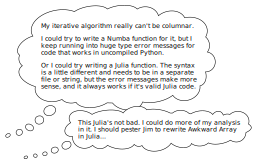
\includegraphics[width=\linewidth]{thought-balloons.pdf}
\end{columns}
\end{frame}

\begin{frame}[fragile]{Conclusion/proposal}
\large
\vspace{0.35 cm}

\begin{enumerate}\setlength{\itemsep}{0.25 cm}
\item<1-> Teach PyJulia to recognize Awkward Arrays (ArrayBuilders?) as arguments.

\item<2-> Minimal runtime representation, e.g.

\small \begin{minted}{julia}
struct AwkwardArrayView{AwkwardNodeType}
  pos::UInt64                 # nesting level (index in arrayptrs)
  start::UInt64 stop::UInt64  # view within this nesting level
  arrayptrs::Ptr{Ptr{Cvoid}}  # to be cast with 'unsafe_wrap'
end                           # total: 32 bytes
\end{minted}

\large
\item<3-> Generate \mintinline{julia}{AwkwardNodeType}-dependent code {\it only for iteration.}

\item<4-> Let physicists choose between \textcolor{darkorange}{\bf Numba} (same as the surrounding language) and \textcolor{darkorange}{\bf Julia} (more consistent, powerful) for non-columnar algorithms.

\item<5-> This may be a ``gateway'' to Julia: strongly motivated (speed), small up-front commitment; encourages physicists to use it more if they like it.
\end{enumerate}

\vspace{0.25 cm}
\uncover<6->{\textcolor{darkblue}{\Large\bf Anyone interested?}}
\end{frame}

\end{document}
